% \begin{table}[h]
% \begin{center}
%      \caption{Índices 1 para casos factíveis}
%      \begin{tabular}{| l | l | l | l |}
%      \hline Índice & LP Petro & LP 2 & Diferença\\ 
%      \hline $SES_y$& 60.5406 & 60.5492 & -0.0087\\
%      \hline $SES_u$& 1166.1464 & 1166.1464 & 2.36*$10^{-9}$ \\
%      \hline
%      \end{tabular}
% \label{table:indices1}
% \end{center}
% \end{table}

\begin{figure}[h]
	\centering
    \begin{subfigure}[b]{0.3\textwidth}
      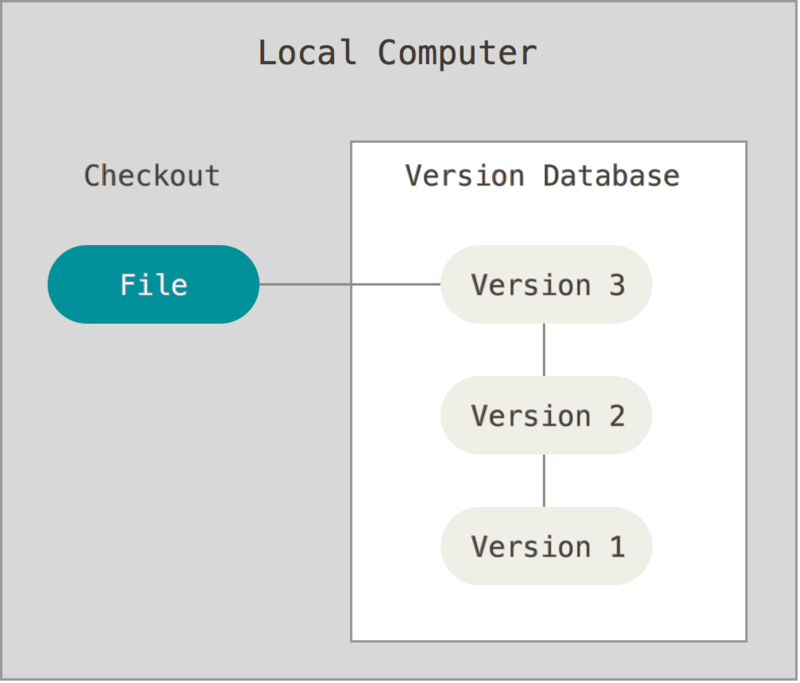
\includegraphics[width=\textwidth]{pfc/figuras/control-version-local.png}
      \caption{Controle local}
      \label{fig:version-control-local}
    \end{subfigure}
    ~
	\begin{subfigure}[b]{0.3\textwidth}
      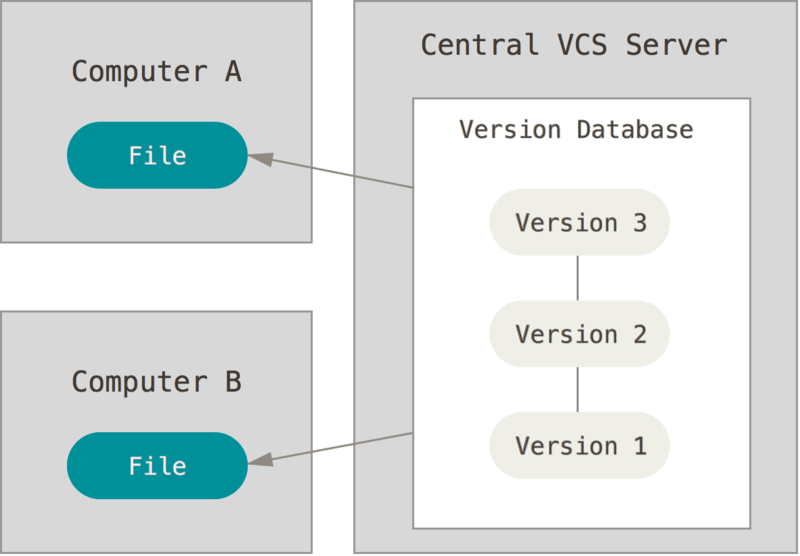
\includegraphics[width=\textwidth]{pfc/figuras/control-version-centralized.png}
      \caption{Controle centralizado}
      \label{fig:version-control-centralized}
    \end{subfigure}
    ~
	\begin{subfigure}[b]{0.3\textwidth}
       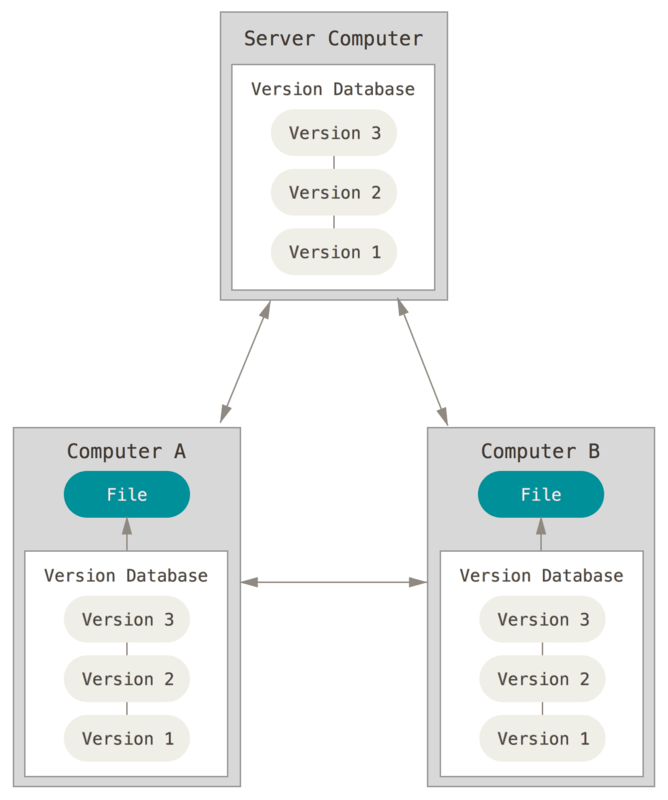
\includegraphics[width=\textwidth]{pfc/figuras/control-version-distributed.png}
       \caption{Controle distribuído}
       \label{fig:version-control-distributed}
    \end{subfigure}
    ~
    \caption{Estratégias de sistemas de controle de versão}
    \label{fig:version-control}
\end{figure}
